\documentclass[a4paper,11pt]{article}
\usepackage[utf8x]{inputenc}
\usepackage{fullpage}
\usepackage{color}
\usepackage{fancybox}
\usepackage{listings}
\usepackage{multicol}
\usepackage{graphicx}
\title{Human Pedestrian Detection using Histograms of Oriented Gradients}
\author{Allan Ortiz and Brad Seefield\\
	CSS 587}

\begin{document}
\maketitle
\begin{abstract}
Detecting humans in images is a difficult task because of the wide range of variability such as pose, 
illumination and backgrounds. However, this is an important task as many industries could benefit from 
reliable human detection (automobiles, law enforcement, etc). A number of methods for detecting humans 
exist that have proven to be somewhat reliable. For our project we wanted to explore one of these methods 
and how it compared to existing techniques. We chose \emph{Human Pedestrian Detection Using Histograms of 
Oriented Gradients} by Navneet Dalal and Bill Triggs\cite{dalal05}. This method proposes a simpler and more reliable 
way of detecting humans. Dalal et al wanted to find a robust feature set that “allows the human form to 
be discriminated cleanly, even in cluttered backgrounds under difficult illumination.” We set out to 
reproduce their results by developing our own implementation that they outline in their paper.
\end{abstract}

\begin{multicols}{2}
\section{Previous Work}
To understand the importance of the preceding work we will briefly discuss some of the existing methods:
\begin{itemize}
  \item A technique involving Haar Wavelets was researched by Papageorgiou et al\cite{Papa00}. 
    The goal of their work was to detect and recognize various classes of objects (faces, automobiles and 
    pedestrians for this experiment). They use Haar Wavelets to “describe an object class in terms of a 
    large set of local oriented intensity differences between adjacent regions.”
  \item Gavrila et al\cite{Gavri04} created a real-time pedestrian detection application by extracting edge images and 
    matched them to a collection of learned examplers using the chamfer distance.
  \item SIFT based feature detection was improved upon by Ke et al\cite{Ke04} by using Principal Components Analysis 
    (PCA) instead of SIFT’s smooth weighted histograms. These PCA-based descriptors “are more distinctive, 
    more robust to image deformations, and more compact than the standard SIFT representation.”
  \item And numerous others.
\end{itemize}
These methods have been fairly successful already but by using Dalal et el's Histograms of Oriented Gradients(HOGs) method
we could potentially arrive at a solution that produces higher performance\footnote
{When we mention performance we are speaking of performance in terms of accuracy. More specifically, one algorithm 
is more performant if it yields fewer false positives and/or a lower miss rate than another algorithm.} 
with a simpler implementation.

\end{multicols}
\begin{figure}[t]
  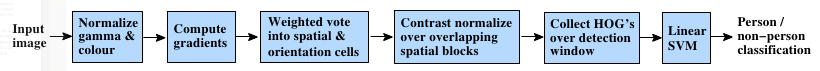
\includegraphics[scale=0.75]{processing_chain.png}
  \caption{HOG processing pipeline}
  \label{HOG_processing_pipeline}
\end{figure}
\begin{multicols}{2}

\section{Approach Outline}
The simplicity of HOGs is that there are no key-points to identify. HOG descriptors are produced from a dense grid 
of uniformly spaced cells. Given an image, the algorithm will divide the image into small spatial regions known as 
cells. A one dimensional histogram of directional gradients is computed for each cell. The cells are grouped into 
blocks. The blocks are normalized by accumulating the local histogram energy and using the results to normalize each 
of the cells in the block. These normalized blocks are what become the Histogram of Oriented Gradient descriptors.
The blocks are overlapped across the detection window so that cells are used multiple times in different 
contexts (we discuss the benefits of this in the results section). The feature vectors are then fed into an 
SVM where a person/non-person classification is made. An overview of the pipeline is shown in 
figure \ref{HOG_processing_pipeline}. 

Dalal et el's experiments showed that color normalization had a small affect on performance. 
In our implementation we used gray scale which had slightly lesser performance than RGB, 
but the implementation is also slight simpler.

\section{Advantages}
Histograms of oriented gradients provide several advantages over the previous approaches. In general the HOGs 
approach provides for a simpler implementation. At the heart of the algorithm is the calculation of gradients 
and their orientation. The remainder of the algorithm is grouping the gradients into blocks and normalizing.

HOGs is robust against translation and rotation so long as the rotation/translation is smaller than the local 
spatial or orientation bin size.

Partial occlusion does not hinder HOG’s ability to identify targets. By using overlapping blocks (a dense grid of cells), 
robust feature descriptors are created that do not rely on the entire target being visible. This is a particular 
advantage over previous methods in which specific key-points had to be visible in order for a positive identification 
to be made. Additionally, by using overlapping blocks a cell is given multiple contexts. For example, perhaps 
a block that yields the correct descriptors for a positive human detection includes both a shoulder and an elbow.
The first block may only include the shoulder, but a subsequent block may include both the should and elbow.

Lastly, but most importantly, Dalal et al showed that HOGs is more performant than the existing methods 
discussed; in some cases, 10-100 times better. They remark that this is ``because none of the key-point 
detectors that we are aware of detect human body structures reliably.'' Intuitively, this makes sense 
given the wide variance of human forms. Relying on specific key-points from one human to the next would not be robust. 

\section{What We Accomplished}
We originally set out to replicate the results of the experiments Dalal et al originally performed in their 
2005 paper. Tangentially, we were trying to better understand how pedestrian detection is performed and what 
are some of the challenges specifically with this kind of detection. This would include creating an 
implementation of their algorithm from scratch, training an SVM and running the experiment with the 
various parameters (e.g., block size, normalization functions, etc).

\section{Implementation}
By design, the HOGs algorithm is not terribly complex. As stated previously, this is one of the benefits 
over existing solutions. Contrary to how Dalal et al developed their implementation, we used 
OpenCV wherever possible. Although writing the code was a straightforward task, verifying correctness 
was more complicated.

One thing we knew going into the project was that we wanted to have unit tests wherever possible. We started 
creating unit tests for methods that had well defined inputs and outputs. As we got further into the 
implementation, unit tests became less effective. We needed to test the result of several methods and 
if the results were visually correct. For example, given an image, are the gradient orientations visually 
correct? A unit test could be written for this, but its a fair amount of setup and we needed a way to test 
many images quickly. We also wanted a way to manually verify the numbers our algorithm was generating. Taking 
inspiration from one of the images referenced in the HOGs paper, we created output images that annotated the 
gradient orientations directly in the image (for each cell). This served its purpose quite well, allowing 
us to visually verify any image that went through the algorithm.

\section{Training the SVM}
Dalal et al used with a linear kernal and we originally anticipated doing the same.
However, after implementing the algorithm using OpenCV, we realized that OpenCV provides an internal 
SVM as well (which shares the common underlying library LibSVM with SVMLight). We chose 
to use the OpenCV SVM out of simplicity.  Using the SVM in OpenCV allowed us to perform all of the 
work in memory, as opposed to having to write the descriptors to file before training or classifying.

We trained the SVM with a set of 90 positive and 90 negative images.  The positive test set contains 
both images and their mirrors. The images are approximately the size of the detection window, 
so we restricted our training to a single centered detection window. The negative test set does not 
contain mirrored images and the images are much larger than the size of the detection window.  
We thus handle the negative training images differently, creating mirrors and then tiling the 
detection window across the image to create a number of detection window sized images.

Unfortunately, as the quarter is short, and training the SVM is long (we settled on 
a configuration that took only an hour for each training), we did not have 
much time to determine the optimal SVM configuration for our application.  
Our choice of SVM parameters is thus unlikely to be optimal.

\end{multicols}
\begin{figure}[t]
  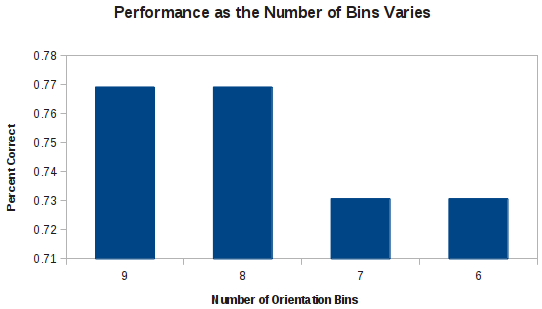
\includegraphics[scale=0.75]{performance_vs_numbins.png}
  \caption{Performance as Number of Orientation Bins Varies}
  \label{NumBins-vs-Performance}
\end{figure}
\begin{multicols}{2}

\section{Experimental Method}
The majority of the project timeline was spent in getting the algorithm to 
work just right and ensuring correct output and training of the SVM. We did 
not reach a state where we could perform large experiments until the final 
day of the project. Because of this, our results section is limited.

\section{Results}
The one experiment that we had time to conduct was to vary the number of orientation bins.
Because varying the number of bins modifies the descriptors generated, we needed to 
retrain the SVM between tests.  Performing the experiment was straightforward:  our 
system is deterministic so no repetitions were needed and only a minor modification 
was needed for each test.  The difficult part of the test was the time cost to retrain the SVM.

As can be seen in figure \ref{NumBins-vs-Performance}, nine bins was found to be the most optimal. This is inline with 
the results that Dalal et al concluded with.

\section{Summary}
The ability to automatically detect humans in a given image has vast applications. Automobiles could use 
it for increasing traffic safety or security organizations could use it to identify people of interest.
However, computer scientists still struggle to produce an accurate and efficient way of detecting humans; even
more so than other types of object recognition. The reason for this is the wide variety of shapes humans can take. 
People are naturally shaped fairly differently, but they can also take on different poses. This makes detection 
quite difficult.

The Histogram of Oriented Gradients attempts to limit the significance of this variance by focusing on smaller 
contexts. By looking at these smaller regions (blocks) we begin to get a more normalized set of descriptors for a human.

Still, the approach makes some very large assumptions. First, we assume the human is standing up right. 
Although we did not test this, we should safely assume that a human who is sitting or laying down 
will not be detected correctly. We hypothesize, however, that this is a fault of the training data and not 
HOGs. Had we trained our SVM with humans in the sitting or laying position, HOGs could perhaps work just as well. 
It would be interesting to see if a single SVM could be used for vastly different positions or if the 
‘noise’ of sitting humans disrupts the accuracy of detecting standing humans. Second, the human accounts 
for a large portion of the window. We did not have time to experiment with this but citing the Dalal et 
al paper, results differed based on the amount of space (padding) surrounded the human. Specifically, 
they found the best results to have 16 pixels of padding around the target (human). Many real-world 
images are not such that a human accounts for the majority of the space. A future implementation could 
likely solve this problem by using varying sizes of windows and sliding the window across the image.

Overall the project was both interesting and challenging. It was interesting to discover the variety of 
methods for detecting pedestrians and realizing that no single solution had yet become a 
'standard’ approach. We were impressed with the simplicity (in hindsight) of the HOGs approach and 
hope that it can continue to be refined so that pedestrian detection can become a reliable problem to solve.
\end{multicols}

\begin{thebibliography}{1}

  \bibitem{dalal05} N. Dalal and B. Triggs. Histograms of oriented gradients for human detection. 
  In CVPR, pages I: 886–893, 2005.

  \bibitem{Papa00} C. Papageorgiou and T. Poggio. A trainable system for object detection. IJCV, 38(1):15-33, 2000.

  \bibitem{Gavri04} D. M. Gavrila, J. Giebel, and S. Munder. Vision-based pedestrian detection: the protector+ system. Proc. of the IEEE Intelligent Vehicles Symposium, Parma, Italy, 2004.

  \bibitem{Ke04} Y. Ke and R. Sukthankar. Pca-sift: A more distinctive representation for local image descriptors. CVPR, Washington, DC, USA, pages 66-75, 2004

\end{thebibliography}


\end{document}